\chapter{Introduction}

% productivity gap
One of the major challenges for the future of semiconductor industry is the problem of overcoming the design productivity gap. This gap is caused by the exponential complexity growth of electronic systems~\cite{Moore_1965_e}  while the capability of design tools cannot cope with this pace, see Fig.~\ref{fig:productivity_gap}. The only way to deal with the increasing complexity of Integrated Circuits (ICs) is to improve the efficiency of the design process, in particular, by heavily reusing system components and by advancing the design automation methods.

\begin{figure}
\centering
   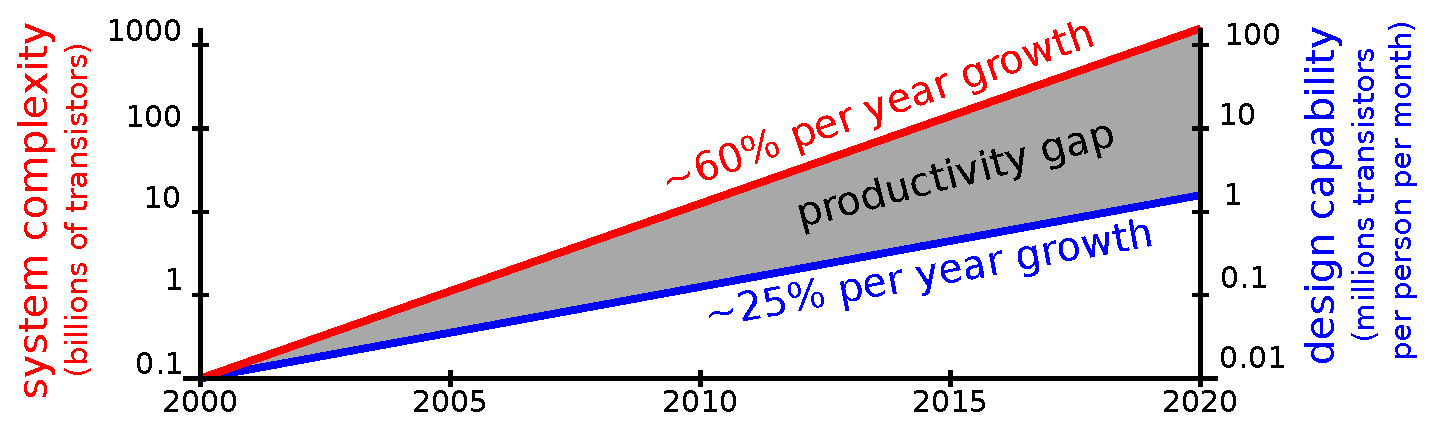
\includegraphics[scale=0.5]{fig/figs/productivity_gap}
   \caption{
     \label{fig:productivity_gap}
     Design productivity gap}
\end{figure}


% design reuse and need for async design principles
It has been predicted by ITRS~\cite{ITRS_2011} that in order to address the productivity gap challenge, by 2020 at least 90\% of the complex circuits should be built of previously designed components. This rises the need for compositional (or modular) design principles where the timing of individual modules is independent of the rest of the system and  therefore requires delay insensitive communication between the modules. This communication discipline is natural for asynchronous circuits where the data transfer is accompanied by request-acknowledgement handshaking between the sending and the receiving counterparts. On this pathway the previously designed Intellectual Property (IP) cores will need to be adapted to the new modular architectures. The least intrusive is the Globally Asynchronous Locally Synchronous (GALS) approach~\cite{Chapiro_1984_phd} where special wrappers~\cite{Mullins_2007_async, Fan_2009_iccd} are built around synchronous modules to convert their communication into asynchronous handshake style. Another alternative is desynchronisation techniques~\cite{Cortadella_2006_ieeetcad} where the global clock is replaced by a distributed control which determines when the computation is complete and the output result is ready to be consumed. This control may take different forms, from a delay line matching the critical path of the module~\cite{Cortadella_2010_icicdt} to explicitly introduced completion detection logic~\cite{Kondratyev_2002_ieeedtc}.

% synthesis of async components
The remaining 10\% of the IC components, as well as the interface and control logic to support the interconnect and communication flexibility, will still need to be designed from scratch. One way is to design those components in traditional synchronous way and then apply the previously discussed techniques to comply with the delay insensitive interface requirements. This, however, may result in suboptimal solutions in terms of circuit area, computation speed and energy consumption. Better results can be achieved if the components are designed and implemented with their asynchronous environment in mind~\cite{Martin_2006_ieeeproc}. However, the logic synthesis of asynchronous circuits is computationally expensive and not applicable to large modules. This is due to high level of concurrency in truly asynchronous systems which results in a state space explosion.  The computation complexity problem has been successfully addressed in the syntax-driven translation~\cite{balsa} approach which is based on direct mapping of a specification into hardware components without going through the state space exploration (it is assumed that there is one-to-one correspondence between the specification language constructs and the library of available components).

% need for compositional approach
The major drawback of the circuits obtained by the syntax-driven translation is the suboptimal performance of their control structures~\cite{Plana-balsa-control-overhead}. In order to resolve this issue the control models of all the components need to be composed together and resynthesised exploiting the benefits of their joint optimisation. Existing resynthesis methods are based on parallel composition of component models expressed in form of Petri nets~\cite{carmona-handshake-clustering}. However, the efficient parallel composition of the component models is still an open question and is one of the primary goals of this thesis.

\begin{figure}
\centering
   \newcommand{\figgg}[2]{
     \subfloat[#1]{
       \label{fig:#2}
       \includegraphics[scale=0.7]{fig/figs/#2}
   }}
   \figgg{Structural composition}{composition_structural}
   \\
   \figgg{Naive behavioural composition}{composition_behavioural_naive}
   \figgg{Behavioural composition}{composition_behavioural}
   \caption{
     \label{fig:composition_basics}
     Composition basics}
\end{figure}

% structural and behavioural aspects of composition
The composition of circuit components is of structural nature - they are combined via input-output interfaces according to the casual dependency between the operation they perform, as shown in Fig.~\ref{fig:composition_structural}.
Another compositional aspect is a combination of several mutually exclusive behaviours in the same circuit. A naive way to build such a circuit is to implement the different behaviour scenarious in separate modules and structurally compose them with the use of multiplexers and demultiplexers, as shown in Fig.~\ref{fig:composition_behavioural_naive}. A mode selection code on the (de)multiplexors determines the current scenario.  While this is a valid implementation of multi-modal functionality, it ignores the mutually exclusive feature of the implemented behaviours and ignores a possibility of partial hardware reuse for common functionality, as shown in Fig.~\ref{fig:composition_behavioural}.

A model which naturally captures the structural and behavioural aspects of composition in a single formalism is Conditional Partial Order Graphs (CPOGs)~\cite{2009_mokhov_phd}. This graph-based model is capable of expressing the structural composition by means of causality arcs (similar to Petri nets) and the behavioural composition by means of Boolean "visibility" conditions on its vertices. While CPOGs is a convenient tool for reasoning on small benchmarks, it lacks the means for capturing and transformation of large systems. The first  goal of this thesis is to generalise the CPOGs model and transition from the acyclic graphs representing partial orders into a universal Parameterised Graphs (PGs). The second goal is to introduce a theory for PG manipulation in algebraic form, which enables equivalence-preserving manipulation of graphs in symbolic form and simplifies specification and reasoning about complex systems.

The Boolean conditions on graph vertices can be expressed in various forms targeting different optimisation criteria. In the context of digital circuit design these conditions are subsequently implemented as the hardware control logic, therefore such optimisation targets as minimising the number of control variables and/or reducing the complexity of logical expressions, is of paramount importance. The ambitious goal of this thesis is to solve the optimisation problem for the general case, to express it in terms of Boolean satisfiability problem and to employ the existing SAT solving tools for obtaining the best result.


\section{Contributions}

The main contributions of the thesis are as follows:

\begin{itemize}
\item
\textbf{Improved parallel composition:} a novel method for composition of models specified with labelled Petri Nets.

\item
\textbf{PG theory:} CPOG generalisation to Parametrised Graph formalism and mechanised proof of its algebraic properties.

\item
\textbf{PG Synthesis:} a technique for synthesis of processor instruction decoder using instruction sets specified with Parametrised Graphs.

\item
\textbf{CAD tool support:} automation for the above, including improved parallel composition and encoding of TPG specifications using Workcraft framework.

\end{itemize}

\section{Overview}

Handshake circuits~\cite{van2004handshake} are widely applied in the design and synthesis of real-life hardware.
One prominent problem is obtaining an efficient implementation from a \emph{structural} compositional specification.
Syntax-based synthesis tools such as Balsa~\cite{balsa} are unable to take into account the compositional
behaviour of STGs corresponding to handshake circuit components. To address this issue we propose 
a technique that selectively composes STGs of related components to obtain a smaller and more performant
circuit without suffering state space explosion commonly associated with Petri net based techniques~\cite{Valmari}.
This transformation, which we refer to as \emph{resynthesis}~\cite{ukaf_balsa_resynthesis,CN-02,KVL-96,PC-96}, is accomplished in three stages. First, we apply a heuristic to identify the most promising candidates for STG-level composition. Second, we perform a parallel composition of the selected component STGs and as a result obtain a new handshake circuit with custom components, functionally equivalent to a combination of elementary components. Finally, a gate-level implementation is obtained from the new handshake circuit via a component-wise synthesis of STGs.

Unfortunately, the standard definition of parallel composition almost always yields a `messy' Petri net, with many implicit places, causing performance deterioration in techniques that are based on structural methods such as the resynthesis approach. To counter this, we propose an improved algorithm for computing the parallel composition. The algorithm generally produces nets with fewer implicit places that are better suited for subsequent application of structural methods~\cite{improved_par_comp}.

In addition to purely structural composition of STGs, it is also beneficial to consider a mixture of 
structural and behavioural composition. Conditional Partial Order Graphs (CPOG)~\cite{2009_mokhov_phd} is a graph-based notation supporting compact
representation and efficient manipulation of both structural and behavioural composition styles. As one example, when developing complex circuit, it is
often necessary to consider several operational modes of a circuit~\cite{2012_xia_iet,2012_mokhov_async}.
For this, one needs methodologies and tools to exploit similarities between
the individual modes and hence lift the level of discourse to behaviour families.
This necessitates that behaviours are managed in a compositional
way: the specification of the system must be composed from specifications
of its blocks. Furthermore, since the approach is intended to be a part of a safety critical toolchain, it is essential that such a  specification is amenable to mechanised reasoning and transformation.

In Chapter~\ref{chap:PGAlgebra} we propose an extension of the CPOG formalism, called Parameterised Graph (PG).
PGs deal with general graphs rather than just partial orders. We introduce an algebra of Parameterised Graphs by specifying the
equivalence relation via a set of axioms, which we prove to be sound,
minimal and complete~\cite{pg_algebra}. This result allows one to manipulate a PG model
as an algebraic expression applying the bi-directional rewrite rules of this algebra. This is  in contrast to the CPOG formalism that does not offer a unifying algebraic structure. We demonstrate
the usefulness of the developed formalism with two case studies coming
from the area of microelectronics design.

The CPOG formalism can be applied to merge several distinct behaviours
into a single compact CPOG~\cite{2009_mokhov_phd}. As one example, this has been previously used to
synthesise control logic for instruction decoding. In this thesis (Chapter~\ref{chap:PGEncoding}) 
we improve upon this work by offering a powerful technique to automatically discover an optimal encoding and
synthesise a matching optimal decoding circuit. From the outset, we consider a larger set of potential solutions
which enables us to formulate the global optimality criterion. We use an automated satisfiability solving 
techniques to find an optimal solution~\cite{cpog_encoding}.

\begin{figure}
\centering
   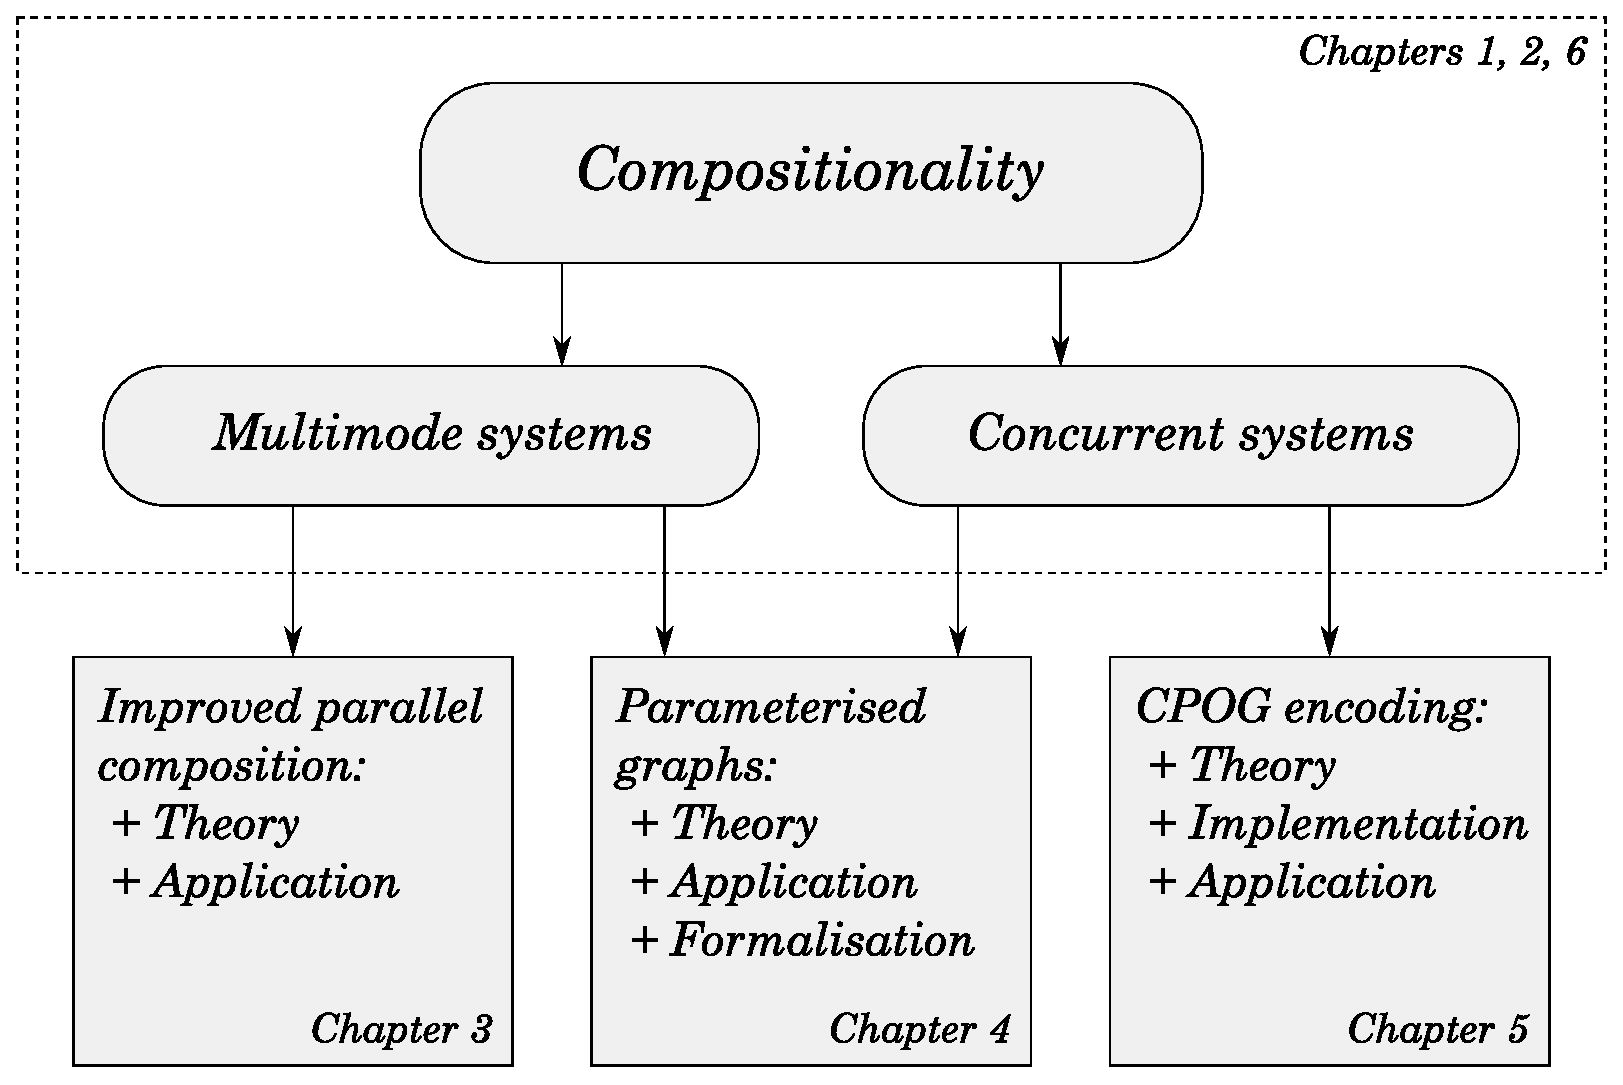
\includegraphics[scale=0.5]{fig/thesis}
   \caption{
     \label{fig:thesis_structure}
     Thesis structure}
\end{figure}

To summarize the thesis structure,

\begin{itemize}
\item
\textbf{Chapter~\ref{chap:Background}} covers the basics of handshake circuits, signal transition graphs and conditional partial order graphs.

\item
\textbf{Chapter~\ref{chap:ParComp}} describes the proposed improved parallel composition algorithm. The contents of this chapter is based on the results published previously in \cite{improved_par_comp}.

\item
\textbf{Chapter~\ref{chap:PGAlgebra}} introduces Parametrised Graph (PG) theory, defining and studying an algebraic structure that generalises Conditional Partial Order Graph formalism. This chapter is based on the results previously published in~\cite{pg_algebra}.

\item
\textbf{Chapter~\ref{chap:PGEncoding}} describes a technique for optimal encoding of processor instruction sets defined using PG formalism. This chapter is based on the results previously published in~\cite{cpog_encoding}. An earlier version of this paper has qualified for a Best Paper Award at the ACSD conference.

\item
\textbf{Chapter~\ref{chap:Conclusion}} summarises the achieved results and proposes ideas for future research.

\item
\textbf{Appendix} contains formal proofs in form of Agda source code for the PG Algebra properties discussed in Chapter~\ref{chap:PGAlgebra}.

\end{itemize}

The relationship between chapters is illustrated in Figure~\ref{fig:thesis_structure}.
